\chapter{Introduction}
\label{sec:intro}


The Standard Model (SM)~\cite{GLASHOW1961579,PhysRevLett.19.1264,PhysRevD.2.1285} of particle physics is a Quantum Field Theory that describes the building blocks of matter and their interactions. It has been developed over several decades from a combination of progress in theoretical physics and experimental discoveries. 

The SM predicts that all matter is composed of a combinations of particles called quarks or leptons and their anti-particles. The interactions between these particles are governed by the strong, weak and electromagnetic forces. 
There are total of 6 quarks and 6 anti-quarks in the SM that can interact via all three forces and there are 6 leptons and 6 anti-leptons however unlike quarks, no leptons can interact via the strong force.

The interactions of each force are described by the exchange of gauge bosons. The electromagnetic force is mediated by the photon, the weak force by the W and Z bosons and the strong force by 8 gluons. 

This final particle in the SM is the Higgs boson. It is interactions with the field associated with this boson that are responsible for the intrinsic masses of the particles.  




The SM can be used to predict how particles will interact and decay. These predictions have been tested in many different experiments over the past decades and so far no significant deviations from the predictions of the SM have been found. 

Although the SM has been shown to be extremely successful there are a number of experimental observations that the SM does not explain. In its current form, the SM cannot explain the observed oscillation of neutrinos from one type into another~\cite{PhysRevLett.20.1205,Fukuda:1998fd, PhysRevLett.86.5656,PhysRevLett.87.071301} and it does not provide a particle or mechanism that could account of the observed presence of dark matter and energy in the universe~\cite{darkmatter1,darkmatter2,Dunkley:2008ie,Ade:2015xua}. Although the SM includes three fundamental forces the final force, the gravitational force, is not included in the formalism of the SM. Furthermore at the start of the universe matter and anti-matter should have been produced in equal amounts but that is not what is observed in the universe today and the SM does not include a mechanism large enough to account to this asymmetry~\cite{Sakharov:1967dj,Gavela:1993ts}.
As well as experimental observations there are more fundamental questions about the SM that are unanswered. There is no reason to explain why there are very large differences in the coupling strengths of the electromagnetic, weak and strong forces or why there is a large range in the masses of quarks and leptons.
The examples given here illustrate that despite the success of the SM it is not enough to describe the universe and indicate that the SM could be a low energy approximation of a more fundamental theory~\cite{lowenergySM}\footnote{A more complete discussion of the shortcomings of the SM can be found in~\cite{Ellis:2002wba}.}.

There exist many theories that go beyond to scope of the SM and seek to explain what the SM cannot. These theories predict the presence of new particles and phenomena that can collectively be called New Physics (NP). However at the moment there is no clear indication of which NP model gives the correct description of the universe and the search for NP effects is ongoing.

The Large Hadron Collider is the latest machine built to study of the predictions SM and to search for NP effects in high energy particle collisions. Two different approaches are used to There are two approaches used search for NP effects at the LHC; direct searches and indirect searches.




Direct searches involve looking for the direct production of on-shell NP particles and phenomena in the data collected from high energy collisions. 
This type of search is limited by the centre-of-mass energy of the collisions that dictates the energy available for the creation of new particles. 
The Higgs boson was found in 2012 by the ALTAS and CMS collaborations using this type of search~\cite{Chatrchyan:2012xdj,Aad:2012tfa} however no new physics effects have been observed from direct searches yet. The lack of observations enables constraints to be placed on the parameter space of NP models.


Indirect searches aim to precisely measure SM processes and look for deviations in the measured values from the predicted values. Deviations can be caused by the presence of NP effects that modify the SM process. 
Indirect searches are not as limited by the centre-of-mass energy of the collisions as direct searches because NP or SM particles influencing these processes are off-shell and therefore lower energy is needed to produce them. In a similar way to direct searches, indirect searches that do not reveal NP effects constraints the parameters space of the theoretical models. Although indirect searches are yet to reveal any significant deviations from SM predictions some interesting anomalies has been seen in the measured results of rare $B$-meson decays by the LHCb, BarBar and Belle experiments. In $b \to sll$ transitions deviations from the SM predictions have been seen in measurements of the angular distribution of $B^0 \to K^{*0} \mu^{+} \mu^{-}$ decays, the branching fraction of $B^{0}_{s} \to \phi  \mu^{+} \mu^{-}$ decays and the ratios $R(K) = \frac{B^+ \to K^+ \mu^{+} \mu^{-}}{B^+ \to K^+ e{+} e^{-}}$ and $R(K^{*}) = \frac{B^0 \to K^{0*} \mu^{+} \mu^{-}}{B^0 \to K^{0*} e{+} e^{-}}$. Also measurements of the ratios $R(D)$ and $R(D^*)$ for the branching fractions of $B^0 \to D^{(*)} \tau^{-} \nu_{\tau}$ and $B^0 \to D^{(*)} \mu^{-} \nu_{\mu}$ are differ from the expected SM values. The individual measurements of these processes are all within 3 standard deviations of the predicted values of the SM however combining the results increases the difference to $\sim 4$ standard deviations for $b \to sll$ transitions, $R(D)$ and $R(D^*)$. Although these deviations are far from conclusive evidence of NP effects, it will be very interesting to see if and how these measurements change in the future.


Particle decays and interactions that are highly suppressed in the SM offer excellent places for indirect searches for NP effects. The possible contributions from NP models can be at a similar order of magnitude to the SM contributions in these decays. The rare decays of $B^{0}$ and $B^{0}_{s}$ mesons into two oppositely charged muons have long been interesting processes through which to test the SM. The purely leptonic final states produces precise theoretical predictions and the 2 muons lave a clearly identifiable signature in particle detectors. The search for \bdmumu and \bsmumu decays began over 30 years ago and over that time the experimental sensitivity to these decays has dramatically increased as illustrated in Figure~\ref{}. The latest experiments to join the search were ATLAS, CMS and the LHCb experiments~\cite{Aad:2012pn,Aaboud:2016ire, Chatrchyan:2011kr, Chatrchyan:2012rga, Chatrchyan:2013bka, Aaij:2011rja, LHCb:2011ac,Aaij:2012ac,Aaij:2012nna,Aaij:2013aka,CMS:2014xfa}. The high energy $pp$ collisions of the LHC has enabled these experiments to reach unprecedented sensitivities to \bmumu decays. 
\begin{figure}[tbp]
    \centering
        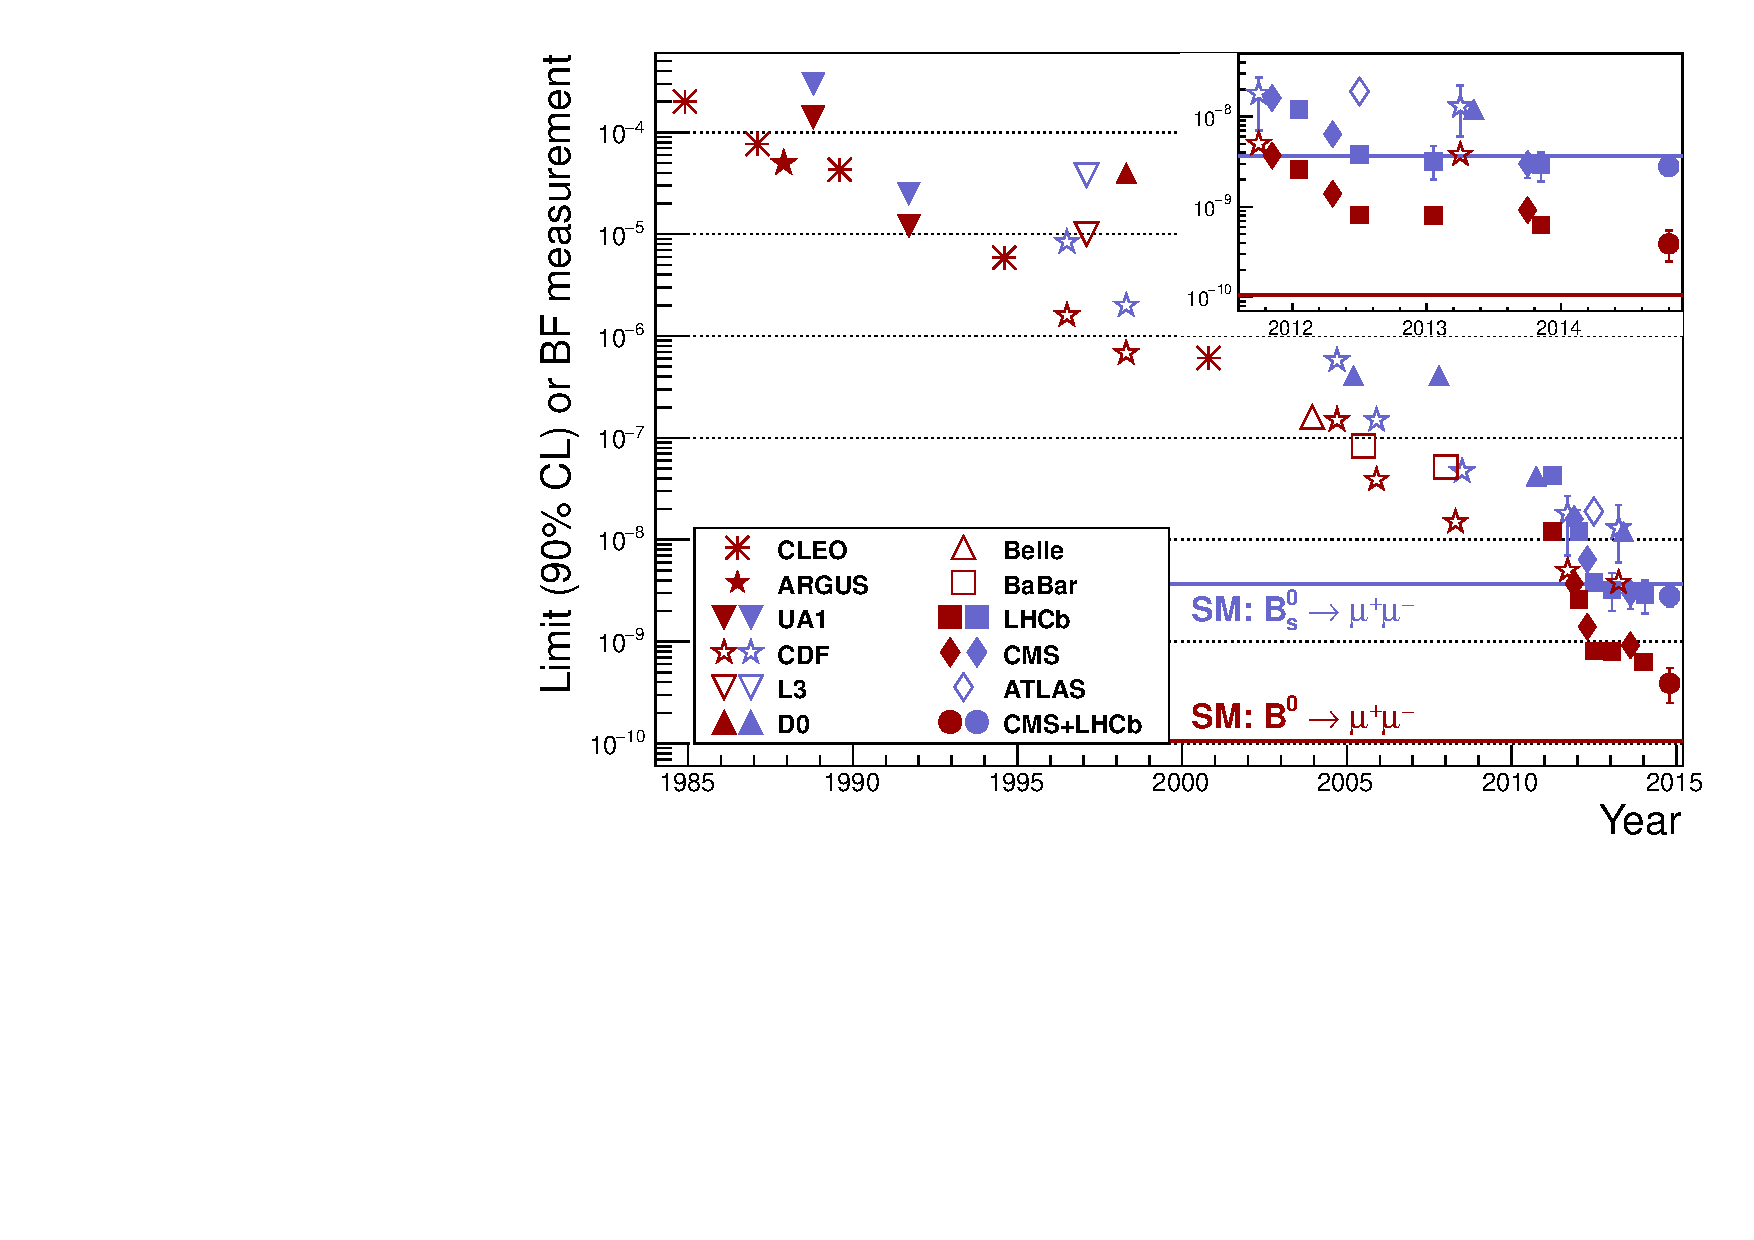
\includegraphics[width=0.8\textwidth]{./Figs/Introduction/CMSLHCb_EDfig7.pdf}
    \caption{Results from searches for \bdmumu (red) and \bsmumu (purple) decays. Upper limits are shown without error bars at the 95$\%$ confindence level. The figure is from reference~\cite{CMS:2014xfa} but updated to include the latest ATLAS result~\cite{Aaboud:2016ire}.}
    \label{fig:bmumu_history}
\end{figure}
The first evidence for \bsmumu decays was found in 2012 by the LHCb experiment~\cite{Aaij:2012nna}. Since then,
the LHCb experiment has measured the \bsmumu \BF to be $\mathcal{B}(B^{0}_{s} \to \mu^+ \mu^-) = (2.9^{+1.1}_{-1.0})\times 10^-9$ at a statistical significance of 4.0$\sigma$ and placed a upper limit on the \bdmumu \BF of $\mathcal{B}(B^{0} \to \mu^+ \mu^-) < 7.4 \times 10^{-10}$ at the 95$\%$ confidence level~\cite{Aaij:2013aka}. The measurements were performed using data collected during 2011 and 2012 at the centre-of-mass energies of 7 and 8 TeV, respectively. Searches for \bmumu decays performed by the CMS experiment using data recorded in the same time period corroborated the results from the results from the LHCb experiment. Producing a measurement of the \bsmumu \BF of $\mathcal{B}(B^{0}_{s} \to \mu^+ \mu^-) = (3.0^{+1.0}_{-0.9})\times 10^-9$ at with a statistical significance of 4.3$\sigma$ and placing a limit on the \bdmumu BF of $\mathcal{B}(B^{0} \to \mu^+ \mu^-) < 1.1 \times 10^{-9}$ at the 95$\%$ confidence level~\cite{Chatrchyan:2013bka}. 
The combined analysis of the CMS and LHCb data sets resulted in the first observation of \bsmumu decays and the first evidence of \bdmumu~\cite{CMS:2014xfa}. The measured branching fractions were measured as
\begin{equation}
\mathcal{B}(B^{0}_{s} \to \mu^+ \mu^-)_{\mathrm{CMS + LHCb}}  = 2.8^{+0.7}_{-0.6} \times 10^{-9}
\end{equation}
\begin{equation}
\mathcal{B}(B^{0} \to \mu^+ \mu^-)_{\mathrm{CMS + LHCb}}  = 3.9^{+1.6}_{-1.4} \times 10^{-10}
\end{equation}
with a statistical significance of 6.2 $\sigma$ for the \bs mode and 3.0 $\sigma$ for the \bd. The ATLAS experiment also searched for \bmumu decay using data collected during the same period~\cite{Aaboud:2016ire}, measuring the \bsmumu \BF as 
\begin{equation}
\mathcal{B}(B^{0}_{s} \to \mu^+ \mu^-)_{\mathrm{ALTAS}}  = 0.9^{+1.1}_{-0.8} \times 10^{-9}
\end{equation}
with a statistical significance of 2~$\sigma$. An upper limit was placed on the \bdmumu decay of $\mathcal{B}(B^{0}_{s} \to \mu^+ \mu^-) >4.2 \times 10^{-10}$ at the 95 $\%$ confidence level.
Although it was hoped that large deviations from the SM predictions would be found in these decays this has not been observed. 
All the measured values are consistent with the expectations of the SM and have enabled constraints to be placed on the parameter space available for new physics models. Nevertheless, the precision of the measurements allows plenty of room for NP effects to be revealed. Furthermore there is some tension between both the separate measurements and each measurement and the SM prediction as shown in Figure~\ref{fig:contour}. 
\begin{figure}[tb]
    \centering
        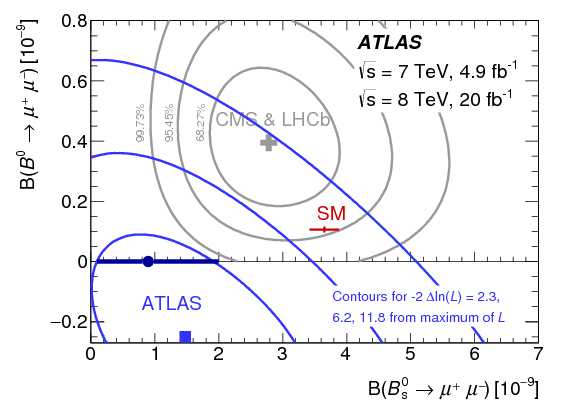
\includegraphics[width=0.8\textwidth]{./Figs/Introduction/contour_plot.png}
        \caption{Measurements of the \bdmumu \BF and \bsmumu \BF from the ATLAS experiment and the combined analysis of CMS and LHCb data alongside the predictions of the SM~\cite{Aaboud:2016ire}. The measurements were performed using data collected during 2011 and 2012 and centre-of-mass energies of 7 and 8~\tev, respectively.}
        \label{fig:contour}
\end{figure}
%The measurements have enabled strong constraints to be placed on the parameter space available for new physics models~\cite{} but the precision of the measurements still allows plenty of room for NP effects to be revealed. 
Therefore the study of \bmumu decays continues to be an very interesting topic in the search for NP effects. 

The data collected during Run 2 of the LHC, where the centre-of-mass energy of $pp$ collisions is increased to 13 TeV, will enable more precise measurements of the \BFs of these decays to be made. 
Furthermore the observation of \bsmumu decays opens the way for other properties of this decay to be studied. In particular the effective lifetime of \bsmumu decays provides a complementary search for NP effects to the \BF measurement, the presence of new physics effects could be revealed in either both or only one of these measurements. The search for \bsmumu decays is over and the study of this decay has begun.



This dissertation documents the latest study of \bmumu decays at the LHCb experiment. The measurements of the \bmumu \BF and the \bsmumu effective lifetime are presented using data collected during $pp$ collisions with centre-of-mass energies of 7, 8 and 13~\tev. The theoretical motivation for studying these decays is given in Chapter~\ref{sec:theory_chptr} and the LHC and LHCb experiment are described in Chapter~\ref{CERN_LHC_LHCb}. The criteria used to identify these decays in the data collected by the LHCb experiment are detailed in Chapter~\ref{selection_chapter} and the measurement of the \BF is briefly covered in Chapter~\ref{sec:BFanalysis}. The measurement of the effective lifetime is discussed in Chapter~\ref{sec:lifetimemeasurement} and the systematic uncertainties on this measurement are given in Chapter~\ref{sec:systematics}. Finally a summary of the results and prospects for future measurements of \bmumu decays are given in Chapter~\ref{sec:summaryandoutlook}.

